

%!TEX root = ./main.tex
\chapter{Of Server Sockets and their Characteristics 
\label{chapter:sockets}}

\section{Server Sockets} Since the Internet has moved from a research project to a widely used, public communication infrastructure, one of the critical success factors was its diversity with respect to network applications or services. This was heavily favored by the Internets layered design as described by the OSI model. 

Todays network applications ranges from traditional services as web, FTP or mail to new and emerging services as video streaming and social networks. However, the term network application or service is overloaded and are differently used depending on the actual technical context.

Since this thesis will operate with flow-level data, layer 5-8 in the OSI model are invisible in the data set. Therefore, network services can be differentiated only by information based on layer 3 and 4 of the OSI model of the two connection end-points. For this reason, the following abstractions of a connection end-point are defined:

%%%%%%%%%%% SOCKET DEFINITION 			%%%%%%%%%%%%%%%%%%%%%%
\parbox{ 
\textwidth}{ 
\begin{defn}
	{\textbf{Socket}\\} A socket is uniquely defined by the triple (\textbf{IP address}, \textbf{IP protocol number} and \textbf{protocol port number}). A socket is only defined for IP protocol TCP(6) and UDP(17). 
\end{defn}
}

%%%%%%%%%%% SERVER SOCKET DEFINITION 	%%%%%%%%%%%%%%%%%%%%%%
\parbox{ 
\textwidth}{ 
\begin{defn}
	{\textbf{Server Socket 
	\label{def:serversocket}}\\} A server socket is a socket with a process listening to incoming connections and thus offering a network service. The lifetime of a server socket is not restricted to individual connections, but by the lifetime of the network service. 
\end{defn}
}

%%%%%%%%%%% CLIENT SOCKET DEFINITION 	%%%%%%%%%%%%%%%%%%%%%%
\parbox{ 
\textwidth}{ 
\begin{defn}
	{\textbf{Client Socket}\\} A client socket is a socket which is only used to initiate a connection to a server socket. Therefore, client sockets are of temporary lifetime which is limited by the duration this connection. 
\end{defn}
}

In spite of the containment of the term \emph{server} in definition \ref{def:serversocket}, this definition is not only valid for server-client application protocols, but also holds for P2P-applications. 
\todo{Explain more?}

\section{Detection of Server Sockets 
\label{section:socket_detection}}

% problem of detection with flow-level information (timing issue + flags)
Basically, a \emph{server socket} can be identified by the fact that a client opens a socket which initiates a connection to a \emph{server socket}. Usually, a \emph{client socket} is chosen at random by his operating system and the \emph{server socket} should be stable over time since it must offer a specific network service or application. Moreover, on each host a socket can only be assigned to one specific process per instance, i.e. a client socket connection initializing application or a \emph{server sockets} network application waiting on client connections. Otherwise, a socket-in-use-error is issued by the operating system. 

A straight-forward approach for detecting \emph{server sockets} is to infer the initiator of the connection by the timing information and determine its opposite as the \emph{server socket}. However, this approach requires a time synchronization of all flow exporting devices across the network. In practice, this can be hardly achieved in a satisfactory and reliable way.

% connection graph idea... +image
Hence, the detection of \emph{server sockets} with flow data relies on the following approach proposed by \citet{Schatzmann:Mining,Schatzmann:Dissection, Schatzmann:Tracing}. First of all, a communication graph is build as shown in figure \ref{fig:bipartite_graph}. This connection graph consists of nodes each representing an unique socket. If a bidirectional connection between two sockets is observed, an undirected, unweighted edge between the corresponding two nodes is assigned. This means that neither the direction nor the weight in terms of packets or bytes are required at all to build the connection graph. 
\begin{figure}
	[h] \centering 
	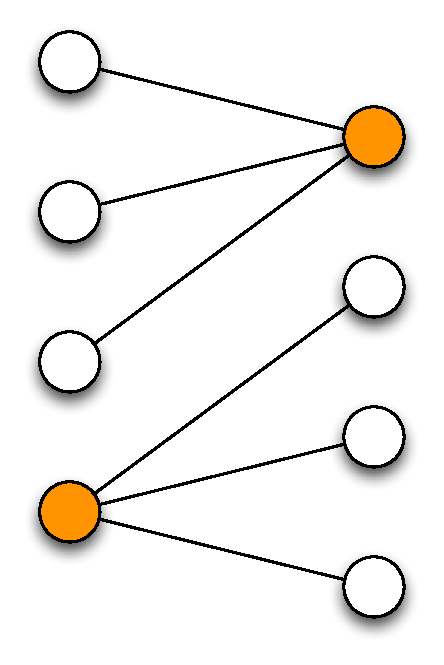
\includegraphics[width=\linewidth/3]{images/connection_graph.eps} \caption{Example of a bipartite connection graph with two concentrators of degree 3 marked as orange} 
	\label{fig:bipartite_graph} 
\end{figure}

In consequence of the fact that \emph{server sockets} provide a network application or service, they are likely to be contacted by several clients depending on their popularity. To this end, a socket which is contacted by a certain amount of client sockets and thus have a high degree in the connection graph is defined to be a \textbf{concentrator}. These concentrators are likely to offer a network service and are thus \emph{server sockets}. 
This approach is able to detect \emph{server sockets} which are offering not only classical client-server services,such as web, FTP, SSH, etc., but also p2p applications such as Skype, Bit-torrent super-nodes, etc. 
Therefore, it can be assumed that nodes with a high degree correspond to a \emph{server sockets}.

% introduce minimal vertex cover problem
\todo{Introduce Minimal vertex cover problem + recall + greedy algorithm}

% greedy algorithm to solve mvcp
% recalling sockets for optimization
\todo{Describe me!}
\begin{algorithm}[t!]
\caption{Detection of server sockets by \citet{Schatzmann:Mining,Schatzmann:Dissection, Schatzmann:Tracing}}
\label{alg:service_tracing_ss-detection}
\begin{algorithmic}
\STATE
\STATE compute list $SS_{in}$ \COMMENT{int. sockets sorted by \# ext. clients}
\STATE compute list $SS_{out}$ \COMMENT{ext. sockets sorted by \# int. clients}
\STATE
\WHILE{(deg($SS_{out}[0]$) $ > 2 $ \OR deg($SS_{in}[0]$)$ > 2$)}
    \WHILE {(deg($SS_{in}[0]$) $ > $ deg($SS_{out}[0]$))}
        \STATE $ss$ = $SS_{in}[0]$ \COMMENT{classify $ss$ as internal server socket}
        \STATE remove $ss$ from $SS_{in}$
        \STATE update deg() for all entries of $SS_{in}$
    \ENDWHILE
    \WHILE{(deg($SS_{out}[0]$) $ \geq $ deg($SS_{in}[0]$))}
        \STATE $ss$ = $SS_{out}[0]$ \COMMENT{classify $ss$ as external server socket}
        \STATE remove $ss$ from $SS_{out}$
        \STATE update deg() for all entries of $SS_{out}$
    \ENDWHILE
\ENDWHILE
\end{algorithmic}
\end{algorithm}

\begin{figure}
	[ht] \centering \missingfigure{Detection Chain}
	
	%\includegraphics[width=\linewidth]{images/detection_chain.eps}
	\caption{Detection chain illustration} 
	\label{fig:detection_chain} 
\end{figure}

\section{Monitoring of Server Sockets 
\label{section:socket_tracking}}

The previous section outlined the approach of detecting \emph{server sockets}. This section covers the approach of monitoring flow data and generating statistical information such that some characteristics and properties of the found \emph{server sockets} can be assessed as outlined in section \ref{section:characterization}.

\subsection{Server Socket Statistics} The monitoring of the external \emph{server sockets} is done with help of the \emph{server socket registry} which is already used in the detection approach. This registry recalls all \emph{server sockets} which are known yet. Hence, all flows originated from a \emph{server socket} or flows which are destined for a \emph{server sockets} are monitored for compiling the socket statistics later used for the characterization.

In contrast to the detection approach, there are no scanning or other noise filters in the processing chain, because of the fact that they will remove at least some flows, mainly unidirectional flows, which are actually relevant for the statistics. 
\begin{figure}
	[ht] \centering \missingfigure{Monitoring Chain}
	
	%\includegraphics[width=\linewidth]{images/monitoring_chain.eps}
	\caption{Monitoring chain illustration} 
	\label{fig:monitoring_chain} 
\end{figure}

Since the processing is based on data containing flows which are active within a certain time slot, the statistics are accounted on a the same discrete time scale, i.e. 10 minutes. 
At first, each flow is checked if it is a flow of a \emph{server socket}. If this is the case, the individual flow statistics are accounted to the corresponding specific server socket \textbf{statistics record}. This includes the following entries: 
\vbox{

%
\begin{itemize}
	\item Number of bidirectional connections 
	\item Number of outgoing unidirectional connections 
	\item Number of incoming unidirectional connections 
\end{itemize}
}

In second step, the statistics records of each discrete time slot are aggregated in such a way that the information of the activity within a certain time slot is kept. Thus, the overall server socket statistics record contains the following entries: 
\vbox{

%
\begin{itemize}
	\item Sum of bidirectional connections of each time slot 
	\item Sum of outgoing unidirectional connections of each time slot 
	\item Sum of incoming unidirectional connections of each time slot 
	\item Number of days with connections 
	\item Number of discrete time slots with connections 
	\item Timestamps of discrete time slots with connections 
\end{itemize}
}

\subsection{Traffic Statistics} Besides of the individual server socket statistics report, overall traffic statistics are accounted, mainly for deducing knowledge of how good the monitoring capability of the server sockets in the registry is. For this reason, each flow which belongs to a server socket which is present in the registry is denoted as monitored. Hence, flows which does not belong to a server socket are accounted as not monitored. 

Moreover, all unmonitored flows can be further investigated for better understanding of the type of this unmonitored traffic. This can be done on the following three scopes: 
\vbox{

%
\begin{itemize}
	\item Protocol level 
	\item Port level for UDP and TCP flows 
	\item Direction 
	\item Type of connection 
\end{itemize}
}

The first scope, covers the problem that server sockets are only defined for protocol TCP and UDP, hence all flows with another protocol are per definition unmonitored.

Secondly, for all unmonitored TCP or UDP flows there is no corresponding server socket in the registry present. There are various reasons for this, mainly related to the detection approach outlined in section \ref{section:socket_detection}. In most of the cases, the sockets are not contacted by enough clients, therefore, the are not detected as concentrators and in consequence of that not denoted as server sockets. Furthermore, scanning activity is also a major contributor to this unmonitored flows, since scanning traffic and other non-legitimate traffic is removed before the server socket detection is performed. Consequently, these scanned sockets are not detected as server sockets, in case there is no legitimate traffic towards these sockets.

On the one hand, there is the possibility to account for each port the unmonitored flows which will lead to very detailed statistical information about the missed server sockets. However, this comes at the price of an inefficient processing and higher memory usage. 

On the other hand, the flows can be categorized by port ranges. In this thesis, there are just two ranges defined for this categorization:

\vbox{

%
\begin{itemize}
	\item Low port: 0-1024 
	\item High port: 1025-65365 
\end{itemize}
}

These categories are further divided by the location of the socket -- internal or external. Hence, the unmonitored TCP and UDP flows or strictly speaking the corresponding socket are accounted by the four categories:

\vbox{

%
\begin{itemize}
	\item external port high, internal port high 
	\item external port high, internal port low 
	\item external port low, internal port high 
	\item external port low, internal port low 
\end{itemize}
}

\section{Characterization of Server Sockets 
\label{section:characterization}} The main interest of this thesis is to characterize \emph{server sockets} by its \textbf{stability}, its \textbf{visibility} and its \textbf{popularity}. These properties tries to address the following characteristics of a server socket:

\vbox{ 
\begin{itemize}
	\item \textbf{Stability:} How stable is the \emph{server socket} regarding its responsiveness or availability: 
	\item \textbf{Visibility:} How frequently is the \emph{server socket} contacted by other socket: 
	\item \textbf{Popularity:} How many distinct sockets are contacting the \emph{server socket}: 
\end{itemize}
}

These three characteristics are directly deducible from the statistics observed by the passive monitoring technique outlined in \ref{section:socket_tracking}. In the following, each of the three characteristics are briefly discussed.

\subsection{Stability of a Server Socket} Because of the definition and its detection approach a \emph{server socket} is offering a bidirectional service which means that the client and the \emph{server socket} are both sending packets. Usually, a client socket is opening the connection to a \emph{server socket} which will reply in return to this request. Generally, this also holds for P2P applications as for example bit torrent. However in this case, there may be two \emph{server sockets} involved in the communication and no client socket. Therefore, a \emph{server socket} -- or the communication of it -- can be characterized as stable if all connections of this \emph{server socket} are \textbf{balanced}. 

%%%%%%%%%%% Balanced Connection DEFINITION 	%%%%%%%%%%%%%%%%%%%%%%
\parbox{ 
\textwidth}{ 
\begin{defn}
	{\textbf{Balanced Connection}\\} A connection between two sockets is balanced, if there is one flow originating from each socket which is destined for the other socket. Hence, the connection is bidirectional. 
\end{defn}
}

Thus, the overall stability \emph{server socket} or availability of its service can be approximated by the ratio of the balanced to all connections destined to this \emph{server socket}, i.e. the balanced and the unbalanced. This ratio is referred as a \emph{server socket} \textbf{stability ratio} and is mathematically defined by equation \ref{eq:ratio}. 
\begin{equation}
	\text{Stability}(\text{Socket}_i) = \frac{\text{balanced connections}(\text{Socket}_i)}{\text{balanced connections}(\text{Socket}_i) + \text{unbalanced connections}_{in}(\text{Socket}_i)} 
	\label{eq:ratio} 
\end{equation}

Hence, a \emph{server socket} with a stability ratio of 1 does only have bidirectional connections and thus, replies to all connection attempts. On the other side, a stability ratio of 0 indicates that there are only connections attempts by client sockets, but the server socket never replied upon these request. Unbalanced outgoing connections from the server sockets are indicating a client error or scanning activities of clients with spoofed (internal) source address which are not observed by the monitoring system. Therefore, these unbalanced outgoing connections are not considered for determining the stability ratio at all.

\subsection{Visibility of a Server Socket}

% discrete time slots activities of a socket, per day, per 5min slot?
% distribution is heavy-tailed, alot of sockets only rarely connected => due to scanning? due to malware?
The monitoring process of the server sockets is done passively, thus if a server socket is visible in the flow level data of a certain time period, the server socket is active during at that time. Hence, the visibility of a server socket during a certain time interval $t+\Delta{t}$ is a binary measure, either inactive in case it is not visible or active in case it is visible in the data set. Equation \ref{eq:visibility} defines the visibility of a socket during the time interval $t+\Delta{t}$: 
\begin{equation}
	\text{Visibility}_t(\text{Socket}_i,t+\Delta{t}) = \left\{ 
	\begin{array}{l l}
		1 & \quad \text{if $\text{Socket}_i$ is active during $t+\Delta{t}$}\\
		0 & \quad \text{if $\text{Socket}_i$ is not active during $t+\Delta{t}$}\\
	\end{array}
	\right. 
	\label{eq:visibility} 
\end{equation}

In consequence, there are different granularities $\Delta{t}$ to define the visibility a server socket. On the one hand, the most fine-grained resolution is just the flow-level data observation period. In most of the cases, this flow-level data observation period is set to 300 seconds. This fine-grained resolution is referred as the \emph{time slot} resolution, since the entire processing is based on such discrete time slotted data, containing all flows active during this time period. 
On the other hand, there are several other more coarse-grained resolutions of the visibility possible. The most obvious is a day long resolution, i.e. $\Delta{t} = 86400$s.

Furthermore, the visibility of a server socket can be extended from a single time period to the overall observation time, i.e. a week long trace, by summing up the individual visibilities of each time slot as shown in equation \ref{eq:visibility_sum}.
\begin{equation}
	\text{Visibility}(\text{Socket}_i) = \sum_{t} \text{Visibility}_t(\text{Socket}_i,t+\Delta{t})
	\label{eq:visibility_sum} 
\end{equation}

However, this summing approach exacerbate the comparison between different observations since it represents the visibility in absolute terms. Therefore, an even better metric for the visibility of a server socket is to average the individual $\text{Visibility}_t(\text{Socket}_i,t+\Delta{t})$ as outlined by equation \ref{eq:visibility_avg}. This normalizes the visibility to a value in the range between 0 and 1, representing the ratio of its visibility to the maximum visibility possible. Thus, a value of 1 means that the socket is visible in every single time slot and a value of 0 that the socket was never active. 
\begin{equation}
	\overline{\text{Visibility}}(\text{Socket}_i) = \frac{\sum_{t} \text{Visibility}_t(\text{Socket}_i,t+\Delta{t})}{\sum_{t}1}
	\label{eq:visibility_avg} 
\end{equation}

\subsection{Popularity of a Server Socket}

% number of flows / clients?.. degree of Server Socket
Besides the visibility of a server socket, its popularity is another major key characteristics. Whereas the visibility of a server socket defines how frequent in time a socket is contacted by at least one connection endpoint, the popularity of a server socket is defined by the number of connection attempts of client sockets during a certain period of time. The popularity of server socket can be deduced by various metrics as the number of flows, bytes or clients.

%% statistics
\newpage
\section{Analysis of Server Sockets in the Wild}

This section covers a detailed analysis of server socket found during a week long data trace from 2010/11/01 till 2010/11/05 -- the first 5 working days in November 2010.

\subsection{Detected Server Sockets}

% sum up of detection parameters > 2 biflows per 5min interval with more TCP packets > 3 UDP > 1

% state overall number of detected external and internal server sockets during this period

\subsection{Server Sockets Flows Gravity}
% traffic statistics of server sockets detected by type and ratio of traffic towards server sockets


\begin{figure}
	[ht] \centering 
	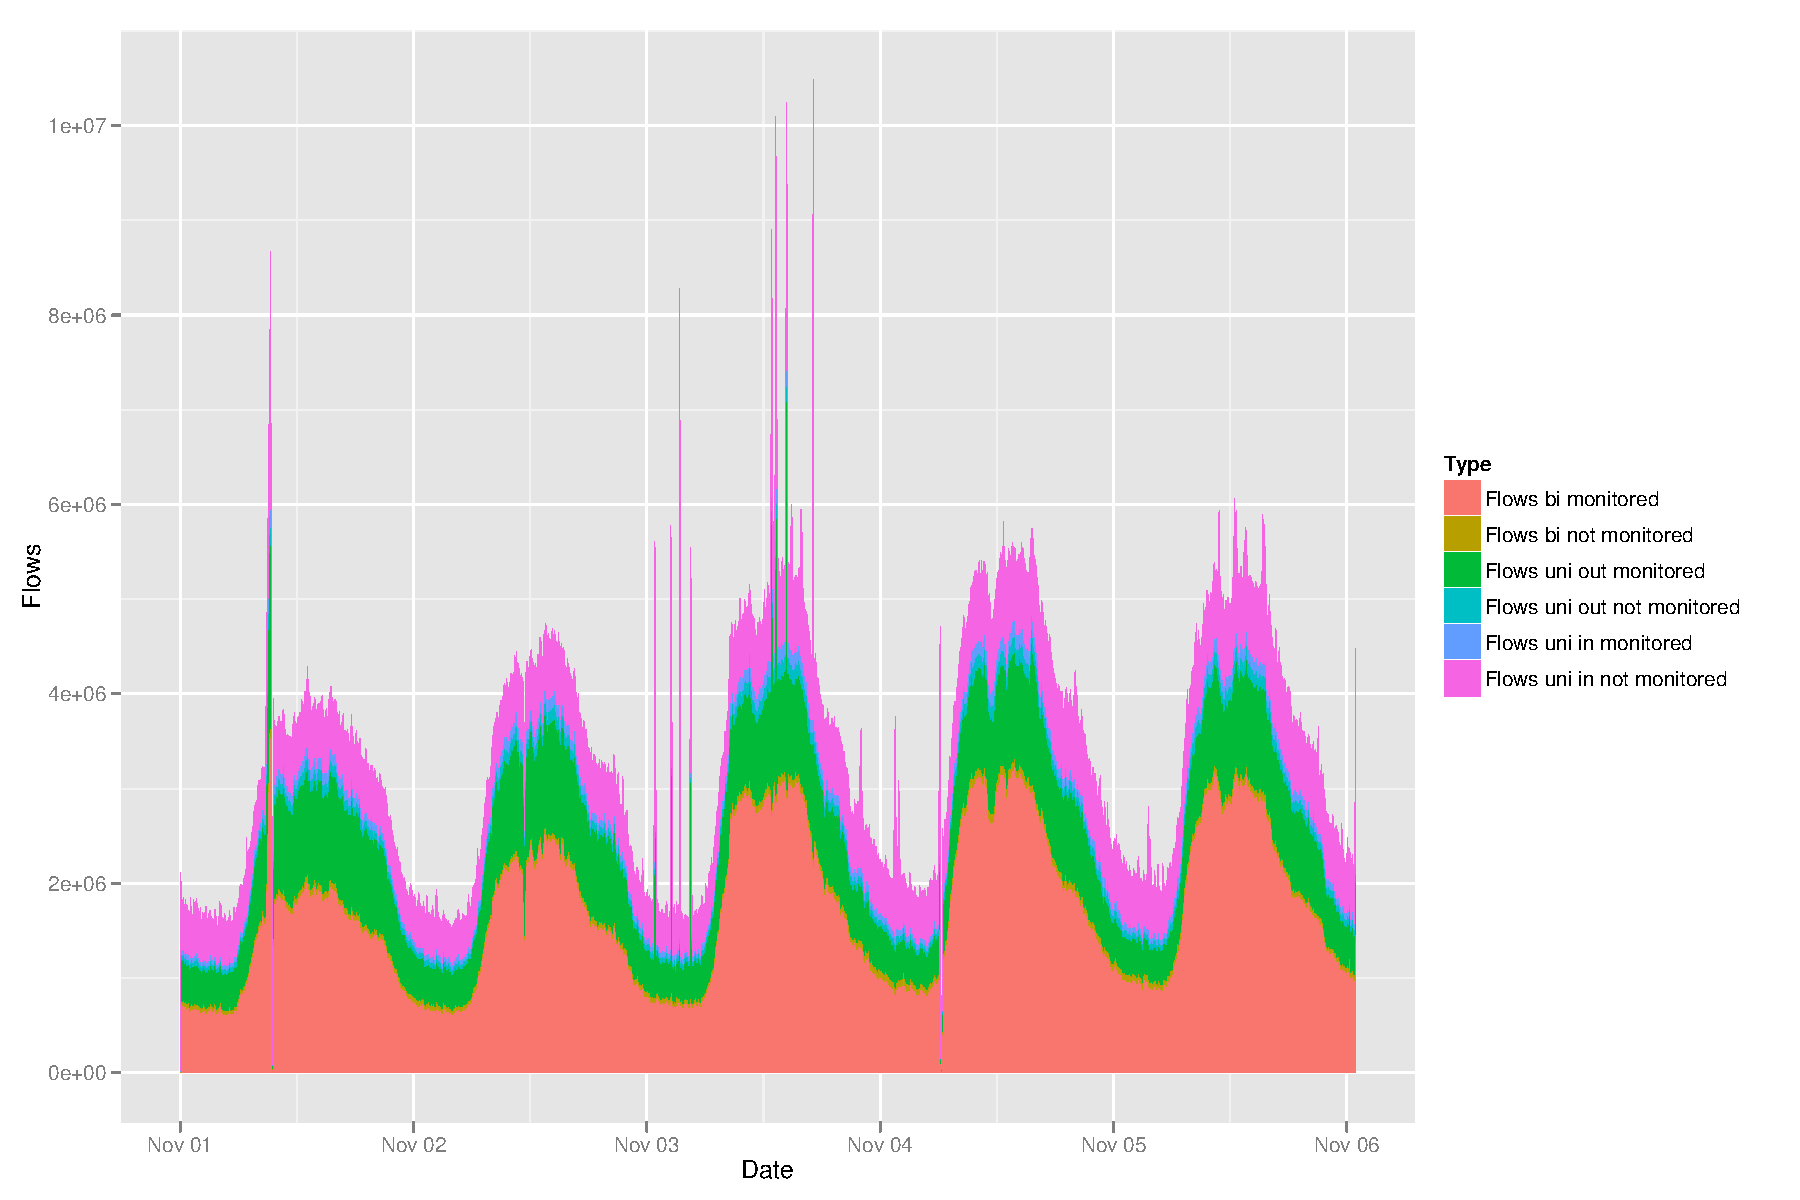
\includegraphics[width=\linewidth]{images/Flows_by_type_area_all_SeS.pdf}
	\caption{Flows by Type} 
	\label{fig:flows_by_type} 
\end{figure}


\begin{figure}
	[ht] \centering 
	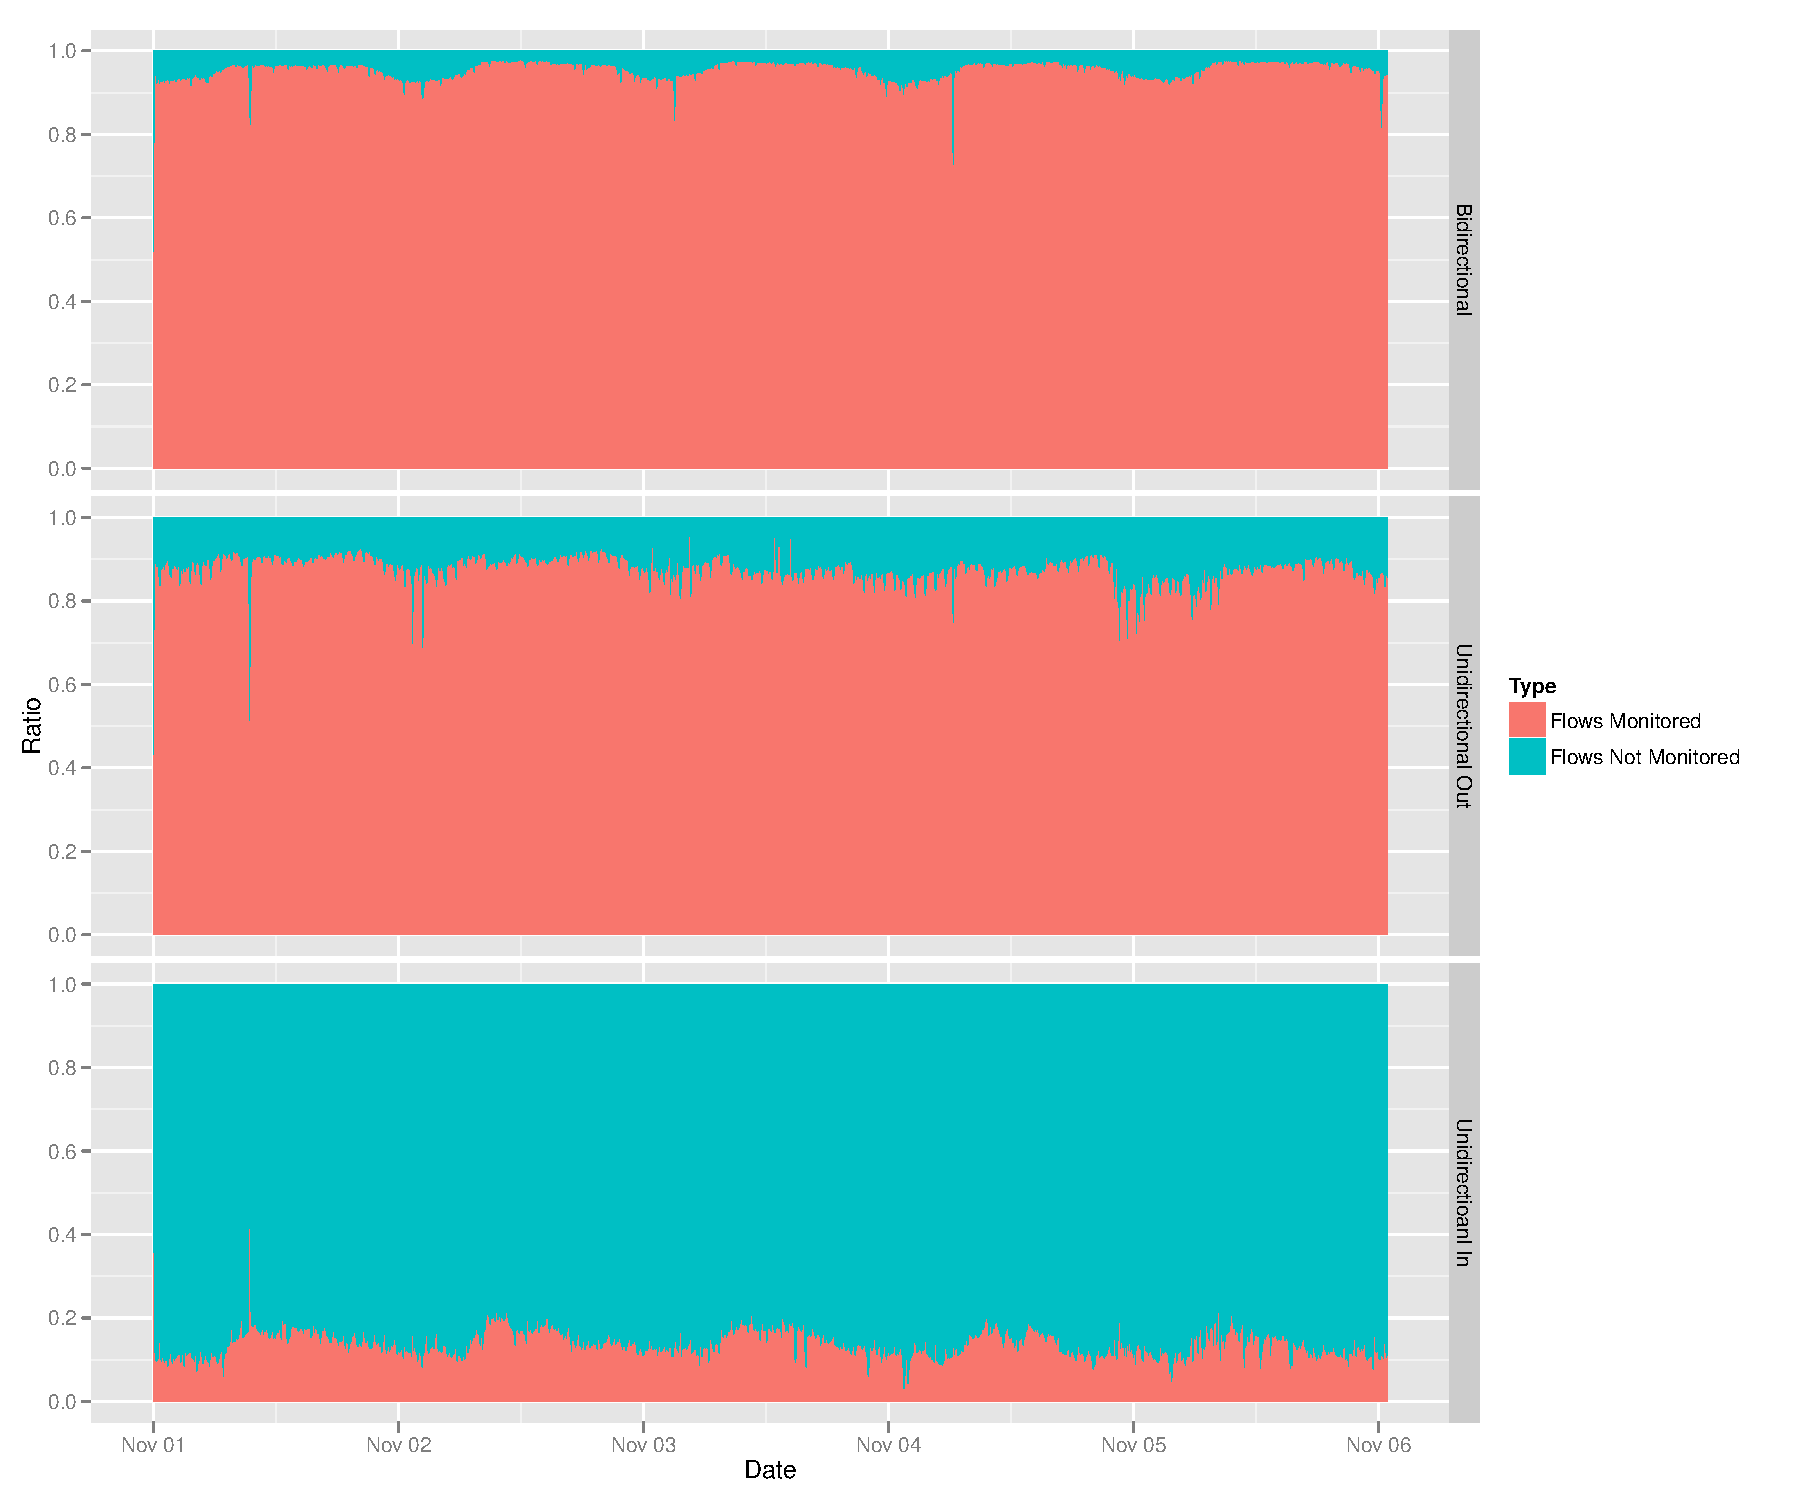
\includegraphics[width=\linewidth]{images/Flows_monitor_ratio_by_type_all_SeS.pdf}
	\caption{Flows towards a detected server socket by type traffic} 
	\label{fig:monitored_flows_by_type} 
\end{figure}


\subsection{Characterization of detected Server Sockets}

\subsubsection{Visibility}
\begin{figure}
	[ht] \centering 
	\includegraphics[width=\linewidth]{images/VTS_by_visibledays.pdf}
	\caption{VTS by visible days} 
	\label{fig:vts_by_visibledays} 
\end{figure}

\subsubsection{Stability}


\begin{landscape}
\begin{figure}
	[ht] \centering 
	\includegraphics[width=\linewidth]{images/CCDF_ratio_days.pdf}
	\caption{CCDF of the availability by visible days} 
	\label{fig:ccdf_ratio_days} 
\end{figure}
\end{landscape}

\begin{landscape}
\begin{figure}
	[ht] \centering 
	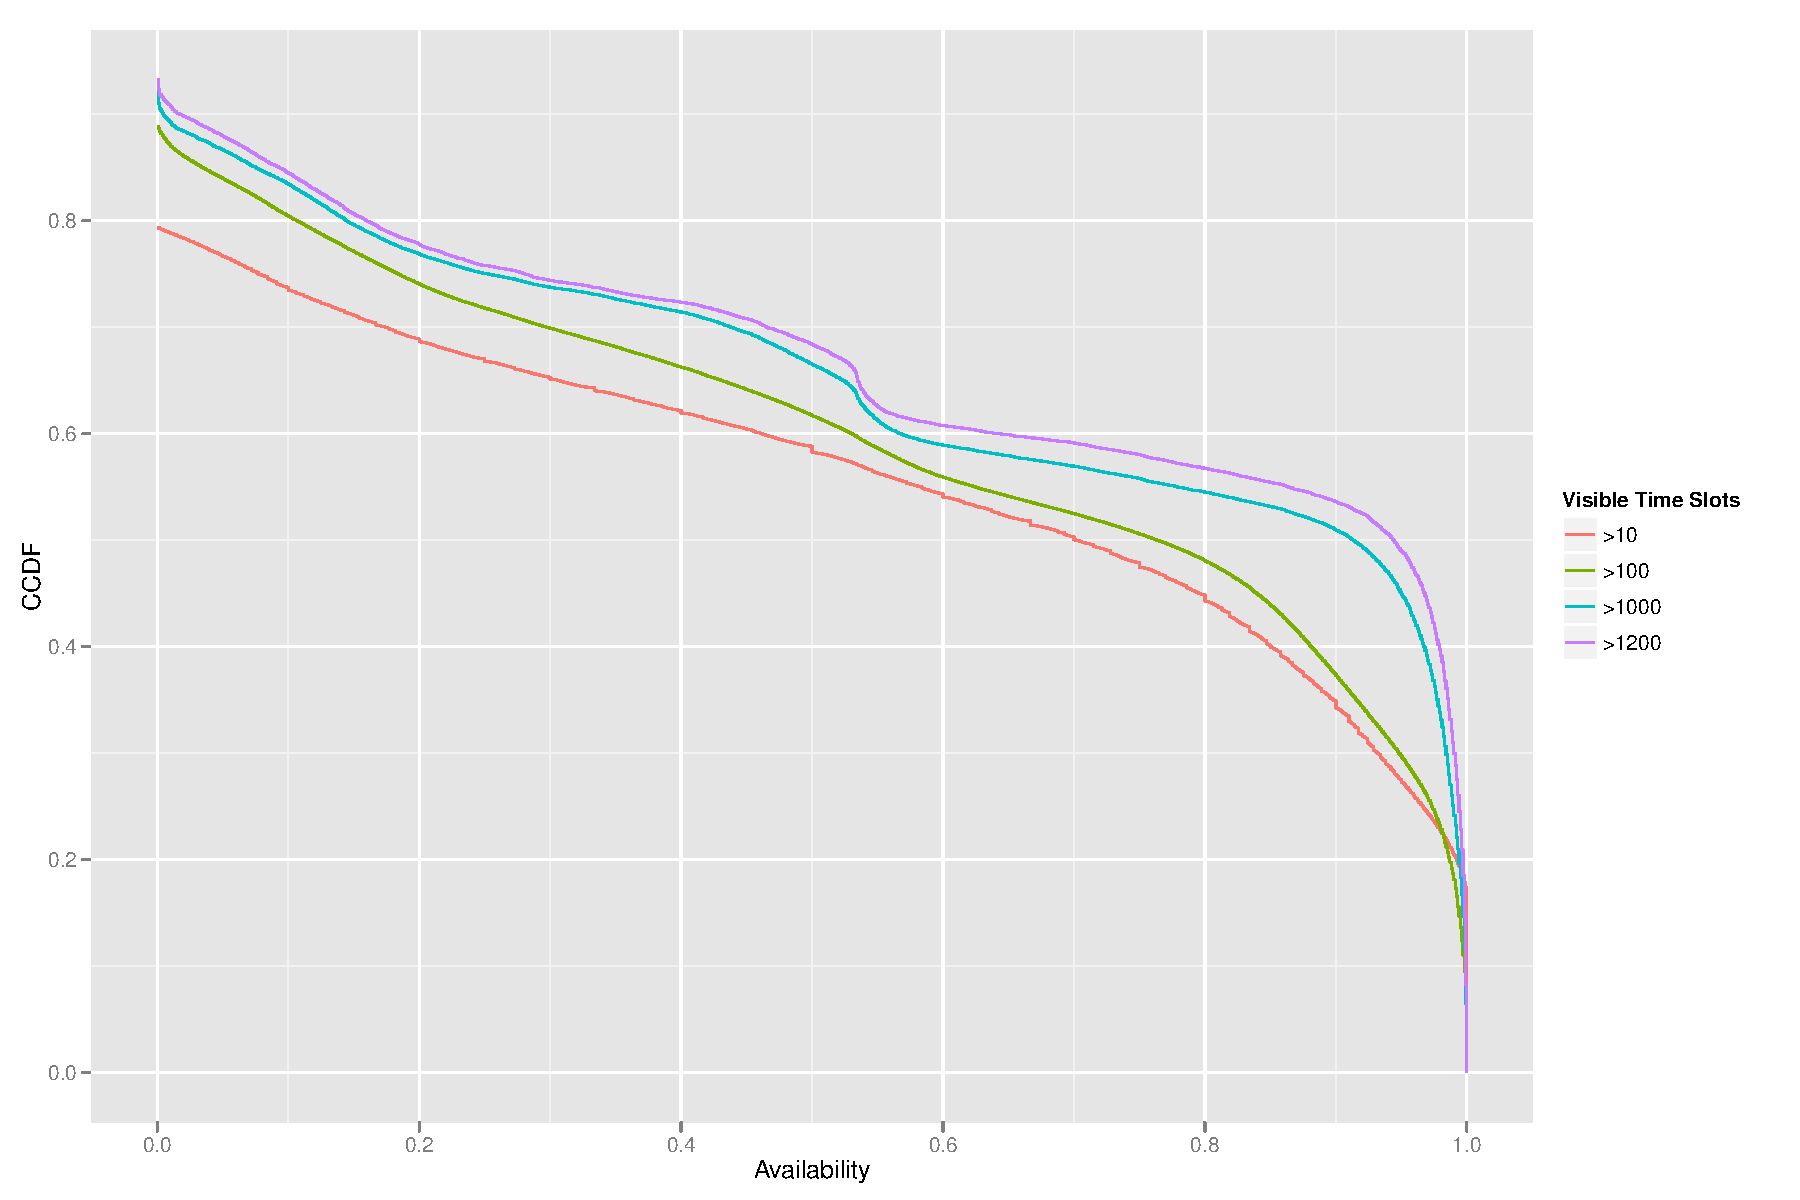
\includegraphics[width=\linewidth]{images/CCDF_ratio_VTS.pdf}
	\caption{CCDF of the availability by visible time slots} 
	\label{fig:ccdf_ratio_vts} 
\end{figure}
\end{landscape}

\subsubsection{Popularity}

\begin{landscape}
\begin{figure}
	[ht] \centering 
	\includegraphics[width=\linewidth]{images/top20_ratio_box.pdf}
	\caption{Boxer plot of the availability / stability of the top 20 traffic port server sockets} 
	\label{fig:top20_ratio_box} 
\end{figure}
\end{landscape}

\begin{landscape}
\begin{figure}
	[ht] \centering 
	\includegraphics[width=\linewidth]{images/top20_visibility_box.pdf}
	\caption{Boxer plot of visibility in days of the top 20 traffic port server sockets}
	\label{fig:top20_visibledays_box}
\end{figure}
\end{landscape}


\begin{table}
	[ht] \centering 
	\begin{tabular}
		{|c|r|r|r|r|r|r|} \hline \textbf{Position} & \textbf{Port} & \textbf{Protocol} & \textbf{Flows} &\textbf{ Flows in \%} & \textbf{Sockets} & \textbf{Sockets in \%}\\
		\hline \hline 1 & 53 & 17 &793851107 & 47.272216 & 314253 & 18.68397\\
		\hline 2 & 80 & 6 &623910956 & 37.152626 & 546735 & 32.50623\\
		\hline 3 & 443 & 6 & 74333936 & 4.426434 & 59800 & 3.555420\\
		\hline 4 & 22 & 6 & 10580812 & 0.630066 & 40363 & 2.399790\\
		\hline 5 & 2703 & 6 & 10139578 & 0.603791 & 22 & 0.001308\\
		\hline 6 & 25 & 6 & 6943533 & 0.413473 & 18560 & 1.103488\\
		\hline 7 & 123 & 17 & 4988781 & 0.297072 & 286 & 0.017004\\
		\hline 8 & 993 & 6 & 3844043 & 0.228905 & 1398 & 0.083118\\
		\hline 9 & 555 & 6 & 3290709 & 0.195955 & 9 & 0.000535\\
		\hline 10 & 995 & 6 & 2411245 & 0.143585 & 654 & 0.038884\\
		\hline 11 & 110 & 6 & 1816240 & 0.108153 & 1211 & 0.072000\\
		\hline 12 & 3789 & 6 & 1796224 & 0.106961 & 10 & 0.000595\\
		\hline 13 & 53 & 6 & 1726716 & 0.102822 & 1102 & 0.065520\\
		\hline 14 & 2128 & 6 & 1677027 & 0.099864 & 390 & 0.023188\\
		\hline 15 & 3478 & 17 & 1607132 & 0.095701 & 176 & 0.010464\\
		\hline 16 & 8080 & 6 & 1362615 & 0.081141 & 2056 & 0.122240\\
		\hline 17 & 3128 & 6 & 1298424 & 0.077319 & 191 & 0.011356\\
		\hline 18 & 5354 & 6 & 1221109 & 0.072715 & 3 & 0.000178\\
		\hline 19 & 8001 & 6 & 1014631 & 0.060419 & 58 & 0.003448\\
		\hline 20 & 21 & 6 & 1010771 & 0.060189 & 1419 & 0.084367\\
		\hline 21 & high & 6 & 37679906 & 2.243762 & 599314 & 35.63233\\
		\hline 22 & high & 17 & 89558306 & 5.333015 & 89820 & 5.340265\\
		\hline 23 & low & 6 & 2505504 & 0.149198 & 3807 & 0.226346\\
		\hline 24 & low & 17 & 749276 & 0.044618 & 302 & 0.017955\\
		\hline 
	\end{tabular}
	\caption{Top 20 port / protocol aggregated sockets by number flows} 
\end{table}

SSH TCP 22: Scanning / PW guessing, e.g. X.X.X.X, 6, 22, 1.0, 2, 1, 69.0, 0.0, 0.0 always with 69 or 68 biflows (parallelized? recurring?) $\rightarrow$ that's way such a bad visibility! one-time shots.. /8 network is scanned! meist 3-4 timeslots und nur visibility einem Tag! 

mDNS (5354) $\rightarrow$ Apple mdns resolving; mainly one socket causing this traffic pm-members.apple.com